%---------- COURSE INFORMATION ------------------------
\newcommand{\course}{CIS 499-01}
\newcommand{\coursetitle}{Indepedent Study - Applied Mathmatics in Computing}
\newcommand{\courseloc}{N/A}
\newcommand{\coursetime}{N/A}
\newcommand{\coursedesc}{Computing topics selected according to the needs of the students.}

\newcommand{\coursesec}{01}
\newcommand{\coursecredithours}{3}
\newcommand{\courseprereq}{Departmental approval.}
\newcommand{\coursedelmethod}{Individual instruction}

\newcommand{\courseobjectives}{\item Explain the relationship between problem solving with both math and computers.
	\item Gain proficiency in common industrial applications that require knowledge of both computing and mathmatics.
	\item Explain the value of mathmatics in applied computing fields.
}

\newcommand{\coursetopics}{\item Math Computer Applications
	\item Scripting Complex Math Problems with Computers
	\item Survey of Emerging Topics in Math and Computing
}
\newcommand{\coursegrades}{Project Work\dotfillsmall 70\% \\
		Final Paper\dotfillsmall 30\% }
\newcommand{\coursetext}{
   No printed textbook required. Various online readings and research.
%	\adjustbox{valign=c}{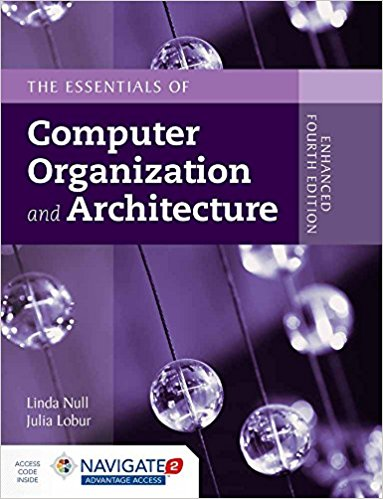
\includegraphics[width=1in]{img/cs490}} & \hangindent .4in \textbf{Textbook:} Null, L., Lobur, J. (2015). Essentials of Computer Organization and Architecture (4th edition). Jones \& Bartlett Learning. ISBN-10: 128407448X, ISBN-13: 978-1284074482. \\
	%& \hangindent .4in Simulation Software: SAM 365 \& 2016 Assessments, Trainings, and Projects with MindTap Reader.
}